%\documentclass[a4paper]{article}
\documentclass[journal]{IEEEtran}

\usepackage[pdftex,pdfauthor={Shabaz Sultan, Chi Chun Wan, Boudewijn Zwaal},pdftitle={Airline sc},colorlinks=true, linkcolor=black,          % color of internal links
    citecolor=black,        % color of links to bibliography
    filecolor=black,      % color of file links
    urlcolor=black   ]{hyperref}
\usepackage[pdftex]{graphicx}
\usepackage{amsmath}
\usepackage{float}
\usepackage{listings}
\usepackage{cite}
\usepackage{tikz}
\usepackage{siunitx}
\usetikzlibrary{shapes.geometric, arrows}
\tikzstyle{startstop} = [rectangle, rounded corners, minimum width=3cm, minimum height=1cm,text centered, draw=black]
\tikzstyle{io} = [trapezium, trapezium left angle=70, trapezium right angle=110, minimum width=3cm, minimum height=1cm, text centered, draw=black]
\tikzstyle{process} = [rectangle, minimum width=3cm, minimum height=1cm, text centered, draw=black]
\tikzstyle{decision} = [diamond, minimum width=3cm, minimum height=1cm, text centered, draw=black]
\tikzstyle{arrow} = [thick,->,>=stealth]

\lstset{language=Python, basicstyle=\ttfamily\scriptsize, breaklines=true}

\author{Team CSB(3)\\Chi Chun Wan -- 2525244 \hspace{0.1\textwidth} Shabaz Sultan -- 2566703 \hspace{0.1\textwidth} Boudewijn Zwaal -- 1897527}
\title{Airline Scheduling with Simulated Annealing}
\begin{document}
\maketitle

\begin{abstract}
\boldmath
The airline scheduling problem is central in the profitability of passenger oriented airlines. Flights are scheduled for a number of planes, subject to several restrictions. We have implemented a simulated annealing algorithm. Novel compared to the literature is the permutation method, which can deal with graphs involving a high number of airports. We have analysed the accuracy of simulated annealing in a one plane scenario and found it settled on the global optimum at a rate of $83\%$. We researched the best homebases using a set of testdata and found Barcelona, Helsinki and Reykjavik for one plane scenario and Lisbon for a six planes scenario as the optimum. 
\end{abstract}

\section{Introduction}
Flight schedules take up a central place in airline businesses. To maximize profit a business has to be as efficient as possible in using its resources and be as effective as possible in meeting marketplace demand. A business wants to plan its flights based on demand, use its airplanes to service these flights as efficiently as possible and assign crews to these flights to minimize expenses. These pose highly complex combinatorial optimization problems that cannot be solved analytically. Instead numerical optimization systems are used and their effectiveness can be influential on the profitability of a passenger focusses airline as a whole.\\
The Dutch airline KLM flies on 150 destinations with 97 airplanes and needs to produce a flight schedule four times a year that maximizes their profitability \cite{Bian2003}. In this paper we will consider this problem in a slightly reduced scenario, with a fictional Mokum Airways that flies on 28 destinations with 6 airplanes. The goal is to maximize profit as measured by revenue passenger kilometers, often used as unit to measure the product being sold in a passenger focussed airline \cite{Schefczyk1993}. In order to obtain the best flight schedule, we use heuristics algorithms to analyze all the possible tours and find the optimal one.\\

\section{Background}
Constructing airline schedules can be broken down in a number of subproblems, each posing a number of computational and algorithmic challenges. Often first the flights that are provided by an airline are constructed, usually subject to complex regulation and non-deterministic customer demand functions. This is referred to as the Airline Scheduling problem in the literature, where the goal is to maximize profits by meeting said demands \cite{Etschmaier1985}. \\
The next step is to assign the flights that are flown to airplanes. This is the so-called Fleet Scheduling Problem \cite{Rushmeier1997}. An airplane schedule can be constructed ahead of time, but scheduling methods for real world scenarios need to deal with real-time adjustments as well due to delays on the day itself (e.g. due to weather conditions, technical problems or issues at an airport). Ideally these schedules are repeatable (usually over either a one or seven day period), requiring that if at the start of the day an aircraft is at airport A, there needs to be an aircraft (not necessarily the exact same, just one of the same type) at airport A at the end of the schedule. \\
Finally crew personnel is assigned to the flights and airplanes. The crew scheduling problem is subject to constraints from flight authority regulation, labour regulation and airline specific regulation and because it represents the largest expenditure for airlines after fuel cost it is an important area of research for the industry as well \cite{Gopalakrishnan2005}.\\
This paper tackles the design and optimization of an airline schedule, with airplane assignment being part of the designed schedule. The one consideration given to the constraints from the crew schedule problem is that the schedule needs to have single homebase, each crew member is assumed to live at said homebase and each plane needs to attend that homebase daily for a crew change.\\
There are various approaches to this problem, such as integer programming \cite{Raff1983} or even agent based approaches \cite{Langerman1997}. One candidate for complex combinatorial optimization problems in general is Simulated Annealing \cite{kirkpatrick1983optimization}. This meta-heuristic has been applied to related problems such as crew scheduling \cite{Sosnowska2001}. It has been specifically used for airline scheduling by \cite{Mashford2001}, which is the main reference for the research described in this paper.
\section{Problem}
We consider an airline with a number of potential destinations and airplanes. The specific dataset used has 28 destinations and potential flights in both directions between every possible pair of destinations. We will analyse the problem with one and six airplanes. We wish to schedule a number of flights over a one day period. Based on the number of passengers and length of the flights a passenger kilometer score can be calculated for each of these flights. The total passenger kilometer score is the metric that needs to be optimized for. The number of passengers are based on a deterministic demand function, where for each potential flight the total passenger demand for the day is provided. \\
The flights are subject to a number of restrictions. In reality there are often regulatory flight restrictions only allowing take-offs and landing at certain hours of the day. We assume a 20 hour period of possible flight and that this 20 hour window is the same for every possible airport. This is a simplification that allows us to ignore timezone considerations. During this period there are a number of things that take up time. The flights will have a variable length of time, based on distance between start and end destination and speed of the aircraft (800 km/h in our example scenario). Docking takes up a certain amount of time (one hour in our example).\\
Beside time the planes' operation is also restricted by fuel consumption. The plane has a certain tank capacity that allows it a certain range before it has to refuel (3199 km in the example). If a plane wants to fly a route without having enough fuel in its tank it needs to refuel first. We will only consider the scenario where refueling will completely fill up the tank and takes up a constant time (one hour). \\
Finally we have two airline requirements. There is the requirement to have the schedule be repeatable. To fulfil this requirement each plane will have its starting airport also be its final destination of the day. The airline also has a certain destination airport designated as homebase, which every plane needs to attend during the day for a crew changeover. 
%To more rigorously define the state-space to be explored we can define a mathematical formalisation. There are multiple formalisations of the problem to be found in the literature. We mostly follow \cite{Mashford2001}, because it most closely matches our research. Let $X$ be the set of nodes representing the airports. $G \subset X \times X$ is the service graph, making up all the valid flightpaths between two airports. In the example scenario we consider this will be the full Cartesian product between all airports, see figure~\ref{fig:service_graph}.
%\\
%\begin{figure}[!h]
%\centering
%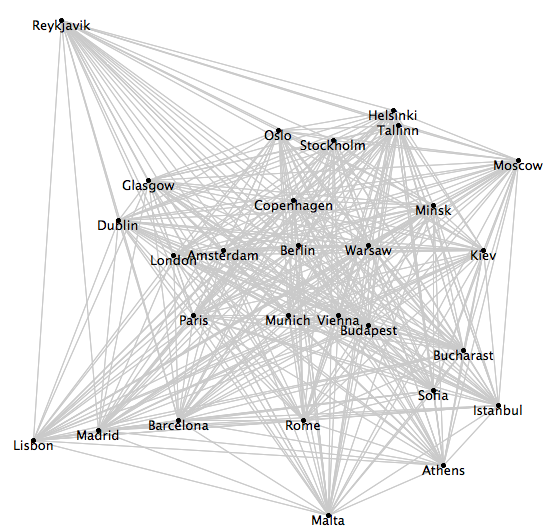
\includegraphics[width=2.3in]{service_graph}
%\caption{Service graph.}
%\label{fig:service_graph}
%\end{figure}
%\\
%We schedule over an interval $[T_1, T_2]$, with $T_1 < T_2$. The fleet is defined as $F = \{p_1 \cdots p_n\}$, with $p_i$ being an airplane. The schedule for a plane is a list of flights, which are defined as quadruples $(x, y, t, p)$, with $x \in X$ the flight origin, $y \in X$ the destination, $t \in [T_1, T_2]$ the departure time and $p\in F$ the plane. \\
%An airline schedule is then defined as [TODO]
\section{Optimisation Algorithms}
The most na\"ive way to approach an optimisation problem is to explore the entire state space and find the optimal solution in said space. We have developed a bruteforce algorithm to do just that, to be used for the simpler one plane scenario where bruteforcing is still computationally feasible. This allows us to apply simulated annealing to the same scenario and quantify its accuracy. We also developed a hill climber based on the same path generation and permutation code designed for the simulated annealer. The latter two algorithms can then be applied the more complex six plane scenario, where it is not computationally feasible anymore to bruteforce. The bruteforcer can be applied greedily to one plane at a time in the six plane scenario to allow for the same performance characteristics as the one plane scenario, but there is a danger of it finding a local optimum. The bruteforcer is however guaranteed to find the global optimum in the one plane scenario.
\subsection{Brute-force}
\label{subsec:bruteforce}
The state space of a plane's flight schedule consists of all possible valid tours. The way the realised brute force algorithm explores this space is by traversing a tree of potentially valid schedules using a depth-first search. This tree is illustrated in figure~\ref{fig:tree}, with the homebase as the the root. Each node in the tree represents a potentially valid tour, each arrow going down being a flight and an additional flight from the node back the root being represented by a dashed grey arrow in figure~\ref{fig:tree}. The depth of the tree is determined by a doing a preliminary check on the validity of each node's schedule. To do this the minimum time taken up by the node's schedule is calculated. We can calculate the time in the air for all the flights represented in the schedule. And if there are $n$ flights, then there are $n-1$ dockings taking up time (the final docking can be outside our time window). And to calculate the time spent refueling the total flight distance is divided by the tank capacity distance (3199 km in our example scenario) and multiplied by the time taken for one refueling (60 minutes). This time can then be checked against the time window a schedule has. This test purposely underestimates the time for the potential schedules. Passing this test does however present a necessary, though not sufficient, condition for being an actually valid schedule. Thus it allows for a tree to be build, where a branch is terminated when it fails this preliminary test. During this preliminary test the flight back to the homebase is discounted, otherwise subtrees are cut that still contain valid schedules, even if the subtree's root node is not valid.\\
\begin{figure}[!h]
\centering
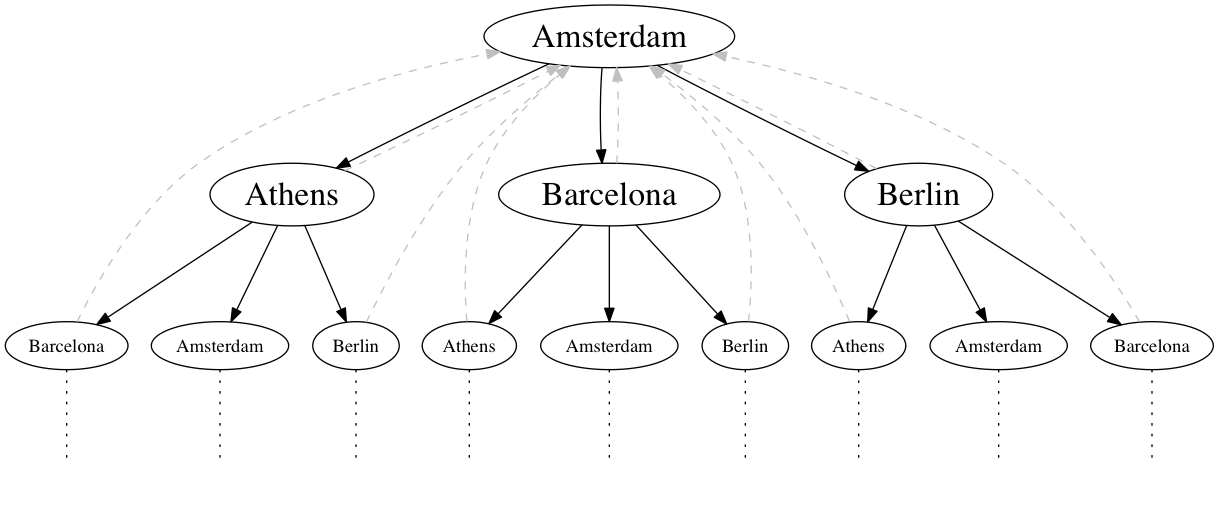
\includegraphics[width=3.0in]{bruteforce_tree}
\caption{Part of a tree representing potentially valid flight schedules in a system with only four cities, with Amsterdam as a homebase.}
\label{fig:tree}
\end{figure}
\\
Attentive readers may have noticed that no consideration is given to the concept of a starting airport of a schedule during tree construction. During the depth-first tree traversal every node visited goes through the first preliminary check. If it passes that check, the actual time spent refueling is calculated. This is done by trying all cities in a potential schedule as starting city and finding which choice of starting city would require the minimum number of refuelings. If the actual refuel time still leads to a total time that fits in the time window the schedule is considered valid. The score is then calculated. If the score is higher than the previous best encountered during tree traversal it is remembered. This will find the global optimum after the entire tree is traversed.\\
While this will works it is still fairly computationally intensive (wallclock time of a couple of hours using a C++ application). To shrink the tree more we can involve the best score found so far during traversal and use it to cut off subtree guaranteed to never produce better scores (i.e. a branch and bound algorithm). For each node a score can be calculated for all flights leading up to said not (not counting the flight back to the tree's root). All these flights will be part of all schedules in the node's subtree. We can also calculate a maximum score still achievable in the subtree of a node. To do this time spend so far getting from the root to the subtree is calculated (using essentially the same calculations as the preliminary schedule validity check). This gives a time left for the subtree. By assuming all the time left is spend in the air, with a plane full of passengers a maximum score that still can be achieved is calculated. If this score plus the score so far is less than the best score found so far the subtree is cut off. (Wallclock time goes down to under a second.)
\subsection{Hill-climbing}
Hill-climbing and simulated annealing share a lot of similarities. They both start with a random solution in state space and iterate on this solution using some permutation method. The permutation method tends to have a stochastic component. The hill-climbing algorithm at each iteration takes the current solution, permutes it and for both solutions calculates a score based on whatever metric is being used for optimisation. It then takes the solution with the best score as input for the next iteration. A schematic overview of the algorithm is presented in figure~\ref{fig:flowchart_hc}.
\\
\begin{figure}[!h]
\centering
%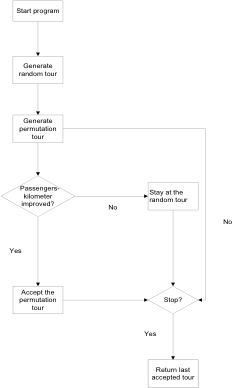
\includegraphics[width=2.5in]{flowchart_hc}
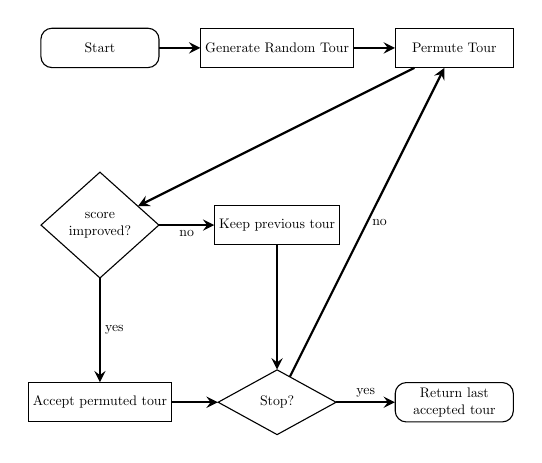
\begin{tikzpicture}[node distance=4.5cm, scale=0.5, every node/.style={scale=0.5, align=center}]
\node (start) [startstop] {Start};
\node (pro1) [process, right of=start] {Generate Random Tour};
\node (pro2) [process, right of=pro1] {Permute Tour};
\node (dec1) [decision, below of=start] {score\\improved?};
\node (pro3) [process, right of=dec1] {Keep previous tour};
\node (pro4) [process, below of=dec1] {Accept permuted tour};
\node (dec2) [decision, right of=pro4] {Stop?};
\node (stop) [startstop, right of=dec2] {Return last\\accepted tour};
\draw [arrow] (start) -- (pro1);
\draw [arrow] (pro1) -- (pro2);
\draw [arrow] (pro2) -- (dec1);
\draw [arrow] (pro3) -- (dec2);
\draw [arrow] (pro4) -- (dec2);
\draw [arrow] (dec1) -- node[right] {yes}(pro4);
\draw [arrow] (dec1) -- node[below] {no}(pro3);
\draw [arrow] (dec2) -- node[right] {no}(pro2);
\draw [arrow] (dec2) -- node[above] {yes}(stop);
\end{tikzpicture}
\caption{Flowchart Hill-climbing}
\label{fig:flowchart_hc}
\end{figure}
\\
\subsubsection{Tour generation and permutation}
To make hill-climbing (and later simulated annealing) work, we need a way to generate tours and to permutate these tours. The way we generate a new tour is as follows. We start in our home-base, and then we add (randomly chosen) cities to the tour until the time is full. Then from the last chosen city we generate a tree-like structure that determines all possible routes from there. If one of those routes lead us back to our home-base within the time window, we accept that one. If such a route does not exist, we cut off the last city of the generated tour and try to reach our home-base again, with the same tree-like structure. If that is not possible again, we cut off the last city one last time and try again. If it is still not possible we try it again with a whole new route. After this we check what would be the most efficient city to start (and end) in, by checking how many times we need to refuel. \\
When permutating a tour, notice that we first shift it such that our home-base is again the first city in the tour. Then we cut off a random amount of cities from the tour (except the first one, which is our home-base). We then try to create a new tour from the two endpoints created in the route. We use the same algorithm for this as we did for the generated tour, i.e. we make a tree of all possible routes from one endpoint and check if one of them leads to the other endpoint. If not we cut off a city and try it again, just as when we generate a random tour. We then again check what is the most efficient start-end city.\\
This tour permutation method is inspired by \cite{Mashford2001}. They however after cutting a part the tour use a set of pre-generated trees that give all possible paths between two tours. They then pick one at random. This is a useful way to ensure that all options to fill up a gap in a tour are possible and that they are all equally likely to be chosen. Pre-generating these trees is however unfeasible for the number of airports we have. The proposed method is a way of hopefully preserving the desired properties of the full tree method, but without having to pre-generate unfeasibly large trees.
\subsubsection{Hill-climbing}
We start with an initial random tour generated with the algorithm described above. To find a better solution, we permutate the tour. The score of the passenger-kilometers for the initial tour is stored in a variable best score. If the score of the permutation tour is higher than the score of the arbitrary tour, the score of the permutated tour will be the new best score and the permutation tour will be accepted, otherwise the best score will stay the same and we will stay at the previous tour. This process is repeated until no further improvements can be found and the best tour is the last accepted tour. When applied to multiple planes, first one of the planes in the system is randomly chosen and its flightplan (tour) is permutated. The total score of all airplane tours is then calculated and compared to the previous best score. If it improves on said score, the new tour is accepted.\\
A disadvantage of hill-climbing is that it is good for finding a local optimum, but it is not guaranteed to find the best possible solution (global optimum). To avoid this disadvantage, we use a different algorithm, simulated annealing. \\
\subsection{Simulated Annealing}
Simulated annealing has the same iterative algorithm properties as the described hill-climber, using the same permutation method during iteration. And like hillclimbing, if a new tour is generated with a better score, it will always be used as input for the next iteration. However, when a permutation is encountered that does not improve the score, there is a chance it is used as input for the next iteration anyway. This allows the simulated annealer to more fully explore state space. The chance of it accepting a worse score is gradually lowered, so that it slowly transitions to a hill-climber, but ideally with a lower chance of it getting stuck in a local optimum than a straight up hill-climber. In figure~\ref{fig:flowchart_sa}, an updated flowchart is presented, where the `score not improved' branch is adjusted according to the simulated annealing algorithm.\\
\begin{figure}[!h]
\centering
%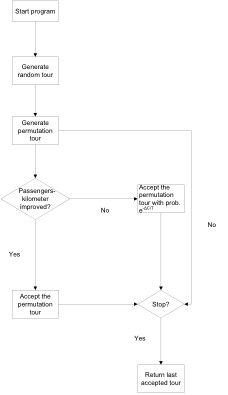
\includegraphics{flowchart_sa}
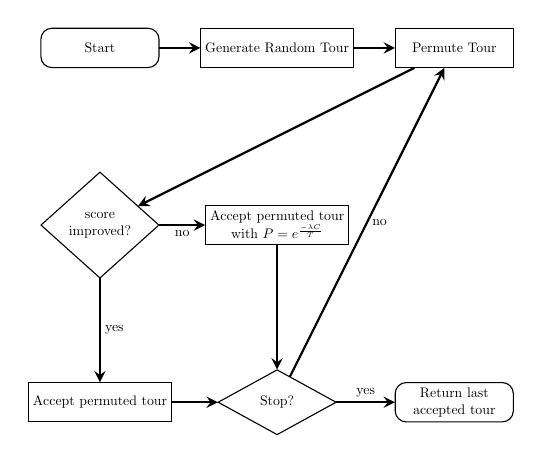
\begin{tikzpicture}[node distance=4.5cm, scale=0.5, every node/.style={scale=0.5, align=center}]
\node (start) [startstop] {Start};
\node (pro1) [process, right of=start] {Generate Random Tour};
\node (pro2) [process, right of=pro1] {Permute Tour};
\node (dec1) [decision, below of=start] {score\\improved?};
\node (pro3) [process, right of=dec1] {Accept permuted tour\\with $P=e^{\frac{-\lambda C}{T}}$};
\node (pro4) [process, below of=dec1] {Accept permuted tour};
\node (dec2) [decision, right of=pro4] {Stop?};
\node (stop) [startstop, right of=dec2] {Return last\\accepted tour};
\draw [arrow] (start) -- (pro1);
\draw [arrow] (pro1) -- (pro2);
\draw [arrow] (pro2) -- (dec1);
\draw [arrow] (pro3) -- (dec2);
\draw [arrow] (pro4) -- (dec2);
\draw [arrow] (dec1) -- node[right] {yes}(pro4);
\draw [arrow] (dec1) -- node[below] {no}(pro3);
\draw [arrow] (dec2) -- node[right] {no}(pro2);
\draw [arrow] (dec2) -- node[above] {yes}(stop);
\end{tikzpicture}

\caption{Flowchart Simulated Annealing}
\label{fig:flowchart_sa}
\end{figure}
\\
In the case when the passengers-kilometer score is not improved, you will accept the permutation tour with probability 
\begin{equation}\label{eq:transition_probability}
P = e^{\frac{−\Delta C}{T}} ,
\end{equation}where the difference in score is 
\begin{equation}
\Delta C = C_{\text{permuted}} - C_{\text{last accepted}}.
\end{equation}
The temperature $T$ is gradually lowered as the iterations $i$ go up, in a logarithmic manner using
\begin{equation}
T = \lambda^i \times T_0,
\end{equation}
with $\lambda$ being the cooling rate (values like $0.999$, $0.9999$, etc. used in our test runs) and $T_0$ the starting temperature. This probability will decrease with the number of iterations. Thus when the number of iterations increases, the temperature goes down. When temperature is high, the system will choose new states more or less at random, but as the temperature lowers this algorithm will go to hill-climbing. 
\section{Results}
%To validate our method, demand and flight distances for a fictional airline are used. Mokum Airways, a newly created Dutch airline based in Amsterdam, has landing rights for 28 destinations around Europe. The airline has a fleet of six Airbus A321 aircrafts with speed of 800km/h, capacity of 199 and range of 3199 km. The take-off and landing take place between 02:00 and 06:00 and docking time and refuel time will take one hour. Moreover, once per day the plane needs to land in the home-base for the crew-change. The flight schedule has to be a cycle, so the start point and the end point of the route has to be the same.\\
%\begin{figure}[!h]
%\centering
%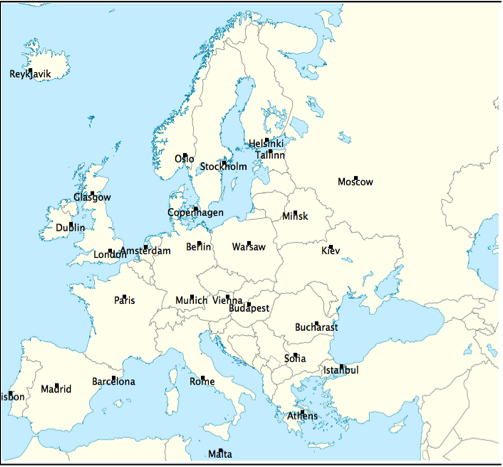
\includegraphics[width=2.5in]{europe}
%\caption{Mokum Airways destinations}
%\label{fig:europe}
%\end{figure}
%\\
The first test scenario involves scheduling one airplane. The first simulations are run to observe general behaviour of the system. In figure~\ref{fig:simulated_annealing_score} the results are plotted for a simulation with initial temperature $T_0=\num{100000}$ and cooling rate $\lambda=0.9999$. We can see that the simulation moves from fairly random to a hill-climber as the temperature lowers. This matches the expected behaviour for simulated annealing and serves as an important sanity check. The second thing to observe is that with a start temperature of $\num{100000}$ the system goes through a significant period of randomness. Ideally we would like to pick a start temperature where the system doesn't have too much randomness and is starting to noticeably transition in its behaviour.\\
There are rigorous methods to do this, where the exact temperature is calculated that leads to a $50\%$ acceptance rate. We have opted to judge things by eye and picked $T_0=\num{50000}$ as our start temperature. For six planes the start temperature is $T_0=\num{50000} \times 6$. The score goes up roughly by six when going to six plane simulations and multiplying the temperature by six roughly preserves the ratio in the exponent of equation~\ref{eq:transition_probability}. The simulations are terminated when there is no change in the accepted schedule for 1000 iterations. \\
\begin{figure}[H]
\centering
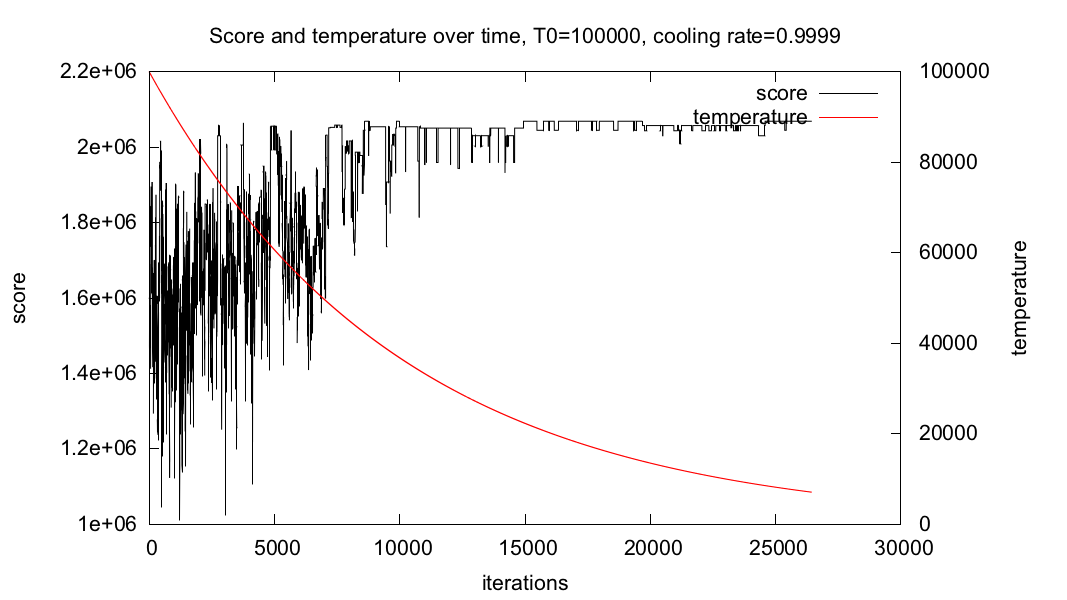
\includegraphics[width=2.5in]{score_over_time}
\caption{Score over time for Simulated Annealing}
\label{fig:simulated_annealing_score}
\end{figure}
\subsection{Best schedule for one plane}
\begin{figure}[!h]
\centering
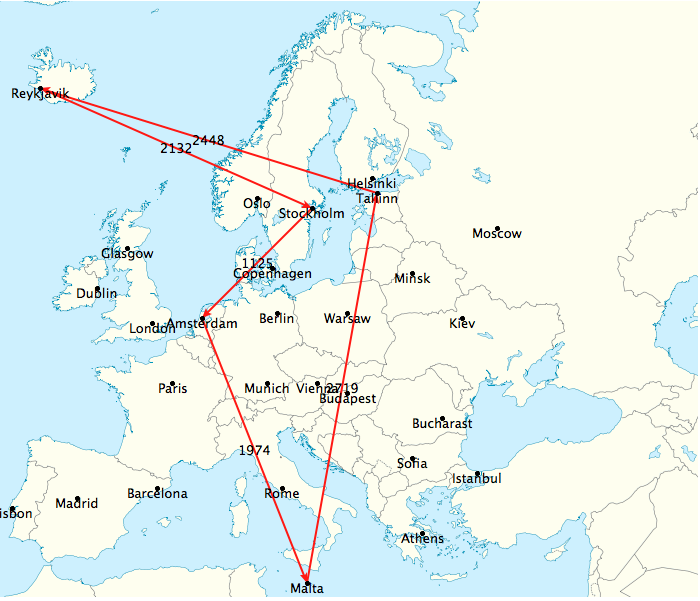
\includegraphics[width=2.0in]{best_tour_one_plane_amsterdam}
\caption{Best tour for one plane with homebase Amsterdam, passenger kilometer score $\num{2069202}$.}
\label{fig:one_plane_amsterdam}
\end{figure}
For scenarios with one plane it is feasible to use a bruteforcer, as described in section~\ref{subsec:bruteforce}. When looking at schedules that have Amsterdam as the homebase, the flightschedule in figure~\ref{fig:one_plane_amsterdam} is found, with a score of $\num{2069202}$. Finding optimal schedules for different homebases can be done by running the bruteforcer with different cities as the homebase. The resulting scores are plotted in figure~\ref{fig:different_homebase_one_plane}. We can see that the best schedule seems to include Barcelona, Helsinki and Reykjavik. This tour is plotted in figure~\ref{fig:one_plane}, with a score of $\num{2195766}$. Any of the three cities can be chosen as start city.
\\
\begin{figure}[!h]
\centering
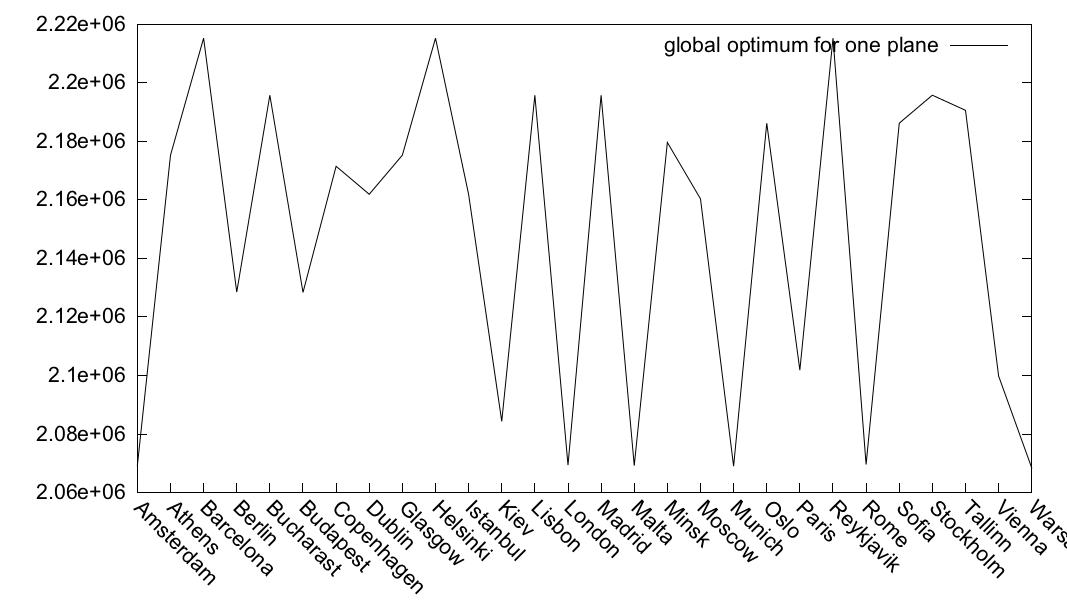
\includegraphics[width=2.5in]{different_homebases_one_plane}
\caption{Global optimum for different homebases with one plane}
\label{fig:different_homebase_one_plane}
\end{figure}
\\
\begin{figure}[!h]
\centering
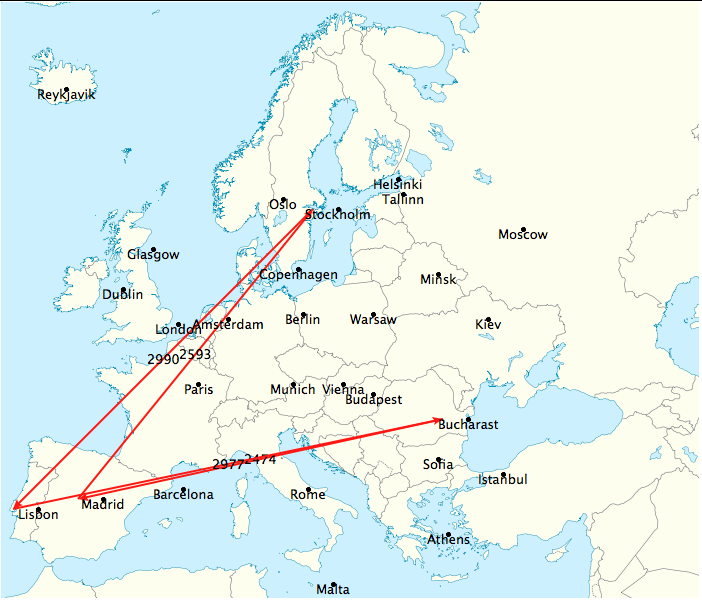
\includegraphics[width=2.0in]{best_tour_one_plane}
\caption{Best tour for one plane with any homebase, passenger kilometer score $\num{2215268}$.}
\label{fig:one_plane}
\end{figure}
To analyze the accuracy of simulated annealing we can use the global optimum as found by bruteforce for one plane with Amsterdam as homebase as reference. We run simulated annealing on the same scenario with a particular cooling rate a hundred times. The results of these testruns are presented in table~\ref{tab:percentage_sa_optimal}. The first thing to notice is that simulated annealing is able to find the global optimum and that it is increasingly likely to find if the cooling rate is slower. This serves as a further sanity check. We also observe that simulation time goes up if the cooling rate is lower. An iteration takes about 4-5ms on our test setup, which means that we move from a run taking roughly a couple seconds for $\lambda=0.99$ to a run taking around 5 minutes with cooling rate $\lambda=0.99999$.
\begin{table}[h]
\centering
\begin{tabular}{lll}
Cooling Rate & Percentage global optimum found & Avg. nr. of iterations(std.dev.) \\
0.99         & 4\%  & 1628.9($\pm 481.9$) \\
0.999        & 6\%  & 2804.3($\pm 1004.3$) \\
0.9999       & 38\% & 13559.6($\pm 5149.9$)  \\
0.99999      & 83\% & 70111.5($\pm 20884.3$)
\end{tabular}
\caption{Percentage of 100 simulated annealing runs finding global optimum, $T_0 = \num{50000}$}
\label{tab:percentage_sa_optimal}
\end{table}
\\
We can further quantify the accuracy of the heuristic by calculating the root-mean-square error (RMSE) of the simulated annealing runs. This is presented as the black line in figure~\ref{fig:error_sa_hc}. We know that simulated annealing can find the global optimum and that if you invest more time by cooling more slowly the probability of finding that optimum go up and the RMSE goes down. We would like to know how effective simulated annealing is in spending its time compared to hill climbing. To this end a hillclimber is run for the same number of iterations as the average iteration counts of various simulated annealing cooling rate. This is presented as the red line in figure~\ref{fig:error_sa_hc}. For each iteration count a hundred runs have been executed. This hill-climber does not have a stop condition (i.e. quiting if the accepted schedule does not change for 1000 iterations). As an alternative the hill-climber is also run with this stop condition turned out, which means it will stop and restart multiple times if the iteration count is high enough. This is represented by the blue line, with again a 100 runs per iteration count.\\
We can see that for the same time investment, simulated annealing tends to have a lower RMSE than both hill-climber plots. This would point at simulated annealing making more effective use of the same time. The simulated annealer is better at avoiding local maxima than even running multiple hill-climbing runs for the same time investment.
\begin{figure}[H]
\centering
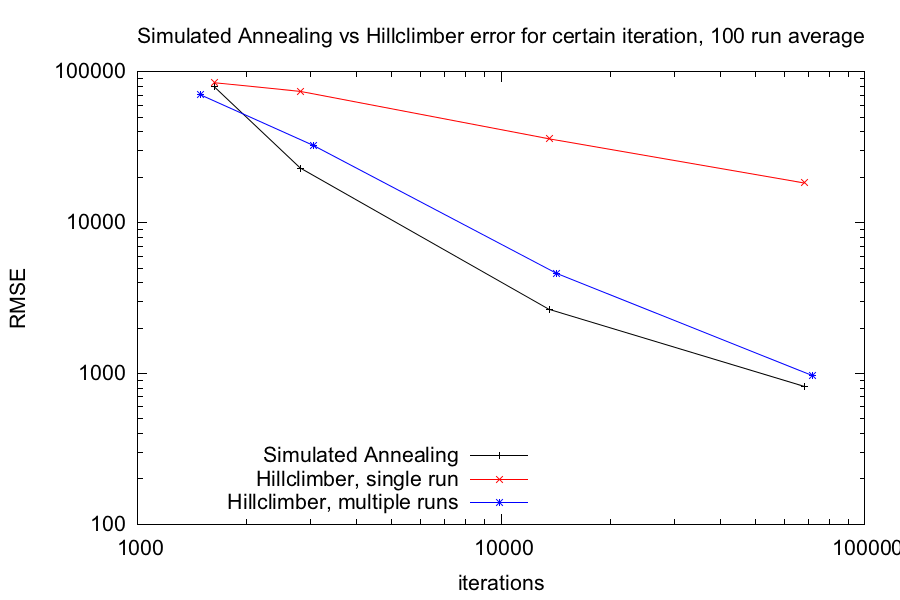
\includegraphics[width=2.5in]{iterations_vs_error_sa_hc}
\caption{Error for Simulated Annealing and Hill-climbing.\tiny}
\label{fig:error_sa_hc}
\end{figure}
\subsection{Best schedules for six planes}
Based on the results for one plane we have selected a cooling rate of $\lambda=0.99999$ for six plane simulations. The best score for six planes with simulated annealing we have found is $\num{12388745}$.  We also have done five simulation runs for every homebase with simulated annealing and six planes. The best score of these simulation runs are plotted in figure~\ref{fig:different_homebase_six_planes} as the blue line. For reference we have also plotted the global optimum times six for the relevant homebases. This serves as a theoretical maximum and is plotted in black.\\
This scenario does not allow for bruteforcing anymore. We can however bruteforce one plane at a time and use it to greedily find schedules for six planes. We bruteforce the first plane and remove the passengers associated with the found schedule from the system. We tend bruteforce the second plane and remove its passengers, etcetera. The results of this greedy bruteforcer are plotted in figure~\ref{fig:different_homebase_six_planes}.  
\\
From these results it seems clear that Lisbon is likely the best choice for a homebase with six planes. There is no way to know if we have found the global optima for the various homebases, but both the greedy bruteforcer and the simulated annealer get the best results using this city. The $28\times5$ simulation runs done to find this result required an average of of 328075.9 (std.dev. $\pm 45001.6$) iterations. Based on 4-5ms per iteration, this requires about half an hour per run.\\
\begin{figure}[!h]
\centering
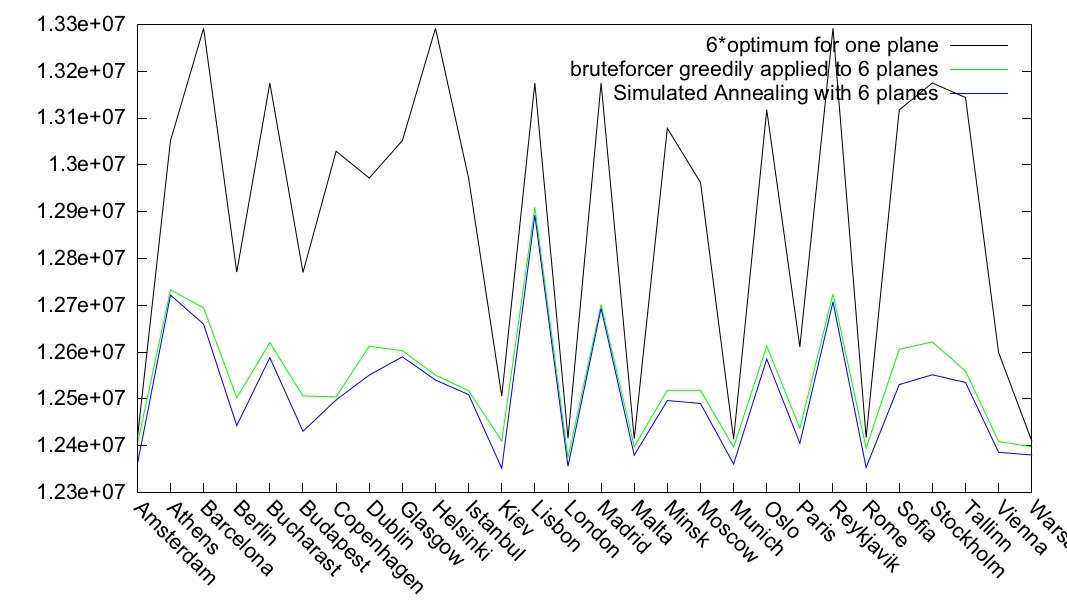
\includegraphics[width=2.5in]{different_homebases}
\caption{Results for different homebases with six planes, Simulated Annealing line based on best of 5 runs for each scenario, cooling rate of $0.99999$.}
\label{fig:different_homebase_six_planes}
\end{figure}
\\
An interesting question to ask is if the single plane solution is at all predictive of the six plane situation in terms of optimal homebase. We know the exact optimal scores for homebases with one plane schedules. And we have two representations that are hopefully indicative of the optimal scores for different homebases with six planes: the results from simulated annealing and greedy bruteforcing. We have calculated a correlation co\"efficient between the optimal scores for one plane and the greedy bruteforcing result, which is 0.832. And the correlation co\"efficient between the six plane simulated annealing runs and the one plane optima is 0.820. This indicates that there is a very strong positive correlation between the optimal homebases for one and sixplanes, even if they do not exactly match. It is thus feasible to assume that finding a very good homebase for a lower number of planes and using this as homebase for more planes will give reasonable results, though likely not optimal.
\section{Discussion}
In our tests simulated annealing either equals or underperforms in terms of score compared to the greedy bruteforcer. One known shortcoming of the greedy bruteforcer is that it can get stuck in a local optimum, where the best set of routes for e.g. six planes does not necessarily contain the best route for one plane. As more planes are added to the test scenario the chance the greedy application of a per-plane bruteforcer encounters a local optimum goes up. And the chance of the difference with the global optimum and the found solution being significant go up as well. In theory a simulated annealer (or other stochastic methods) should be better able to deal with this problem. It would be useful to research the behaviour of the greedy bruteforcer and the simulated annealer applied to scenarios with a lot more than six planes. \\
We speculate that this may be the reason that \cite{Mashford2001} tested only with a scenario containing a high number of aircraft (46) and a low number of airports (12). This maximizes the probability that other methods get stuck in local maxima. The low number of airports also allows \cite{Mashford2001} to go with a relatively simple route permutation algorithm, where all possible routes are enumerated between two points and one is chosen. As the number of airports go up the number of paths becomes infeasibly large. These assumption are not made explicit by \cite{Mashford2001}, but our efforts in partially replicating their methods make us propose these may be unstated reasons for their validation scenario choice. \\
While we do not generate a full tree of all possible paths possible between two airports like \cite{Mashford2001} for our path permutation code, we do have tree generation be a part of our algorithm. In the current version these trees are generated on-the-fly during each path permutation. An obvious candidate for performance optimization is to at least pre-generate a tree with a smaller time limit as bounding function. This could then possibly be integrated in the code so that generating code can be replaced by lookup code; an obvious application of the memoization optimisation technique. \\
Both the hill-climber and the simulated annealer use a Markov chain to traverse the state space of possible schedules. The Hastings-Metropolis algorithm allows you to sample the space stochastically even when the underlying probability distribution is unknown \cite{Hasting1970}. To show that the Markov chain is able to generate all possible paths it is necessary to prove ergodicity; i.e. to prove that the Markov chain is both irreducible and aperiodic. And to make sure that the application of Hastings-Metropolis that is part of simulated annealing is valid it should be shown that every possible `neighbour' state is equally likely to be generated when permuting any of the possible routes. Proving both would be necessary if we're interested in showing theoretical correctness in further research. \\
Finally we have done some exploratory work on applying Genetic Algorithms to this problem. The main challenge is constructing a method of creating new paths with two or more paths as its parents, with some additional mutation. This is equivalent to the construction of a permutation method being the primary challenge of applying a simulated annealing algorithm to a problem. From our literature study there are papers suggesting this approach to the airline scheduling problem and papers applying it to related problems like crew scheduling  (e.g. \cite{Levine1996}). But there is no literature actually applying it to the airline scheduling problem, so this may be interesting area of unexplored research.

%beter variant of greedy

%cooling rate

%50% acceptance, start temp.

\section{Conclusions}
It has been possible to build a simulated annealing based algorithm that can solve the airline scheduling problem. To this end a schedule permutation method was developed that is novel. The simulated annealing method makes more effective use of time than hill climbing, because it does not get stuck in local optima as easily. We have found the global optimum for one plane with a homebase Amsterdam to have a passenger kilometer score of $\num{2069202}$. The best homebases for one planes are Barcelona, Helsinki and Reykjavik, with a schedule involving said cities with a score of $\num{2195766}$. For six planes the best homebase likely is Lisbon. The best result for six planes with homebase Amsterdam from simulated annealing is $\num{12388745}$ and from greedy bruteforcing is $\num{12403073}$. We speculate that the simulated annealer will be more likely to outperform the greedy bruteforcer with more plane, but this has not been showcased in our findings thus far.
\bibliographystyle{IEEEtran}
\bibliography{final_report}
\end{document}

